\documentclass[debug,a0paper,portrait,persian]{xebaposter}

\usepackage{url}
\usepackage{amsmath}
\usepackage{amssymb}
\usepackage{relsize} % for \smaller
\usepackage{graphicx}
\usepackage{multicol}
\usepackage{xecolor}
\usepackage{wrapfig}
\graphicspath{{images/}}
\usepackage[inline]{enumitem}% for making inline list.
\setlist{noitemsep}% Save space in lists.


\usepackage{ptext}
\usepackage{xepersian}
\settextfont{Yas}

%\usepackage{geometry}
%\geometry{papersize={90cm,170cm},verbose=ture,reset}
 %%%%%%%%%%%%%%%%%%%%%%%%%%%%%%%%%%%%%%%%%%%%%%%%%%%%%%%%%%%%%%%%%%%%%%%%%%%%%%%%
 %%%% Some math symbols used in the text
 %%%%%%%%%%%%%%%%%%%%%%%%%%%%%%%%%%%%%%%%%%%%%%%%%%%%%%%%%%%%%%%%%%%%%%%%%%%%%%%%
 % Format 
% \newcommand{\RotUP}[1]{\begin{sideways}#1\end{sideways}}
 %%%%%%%%%%%%%%%%%%%%%%%%%%%%%%%%%%%%%%%%%%%%%%%%%%%%%%%%%%%%%%%%%%%%%%%%%%%%%%%%
 % Multicol Settings
 %%%%%%%%%%%%%%%%%%%%%%%%%%%%%%%%%%%%%%%%%%%%%%%%%%%%%%%%%%%%%%%%%%%%%%%%%%%%%%%%
% \setlength{\columnsep}{0.7em}
% \setlength{\columnseprule}{0mm}

%% Begin of Document
%%%%%%%%%%%%%%%%%%%%%%%%%%%%%%%%%%%%%%%%%%%%%%%%%%%%%%%%%%%%%%%%%%%%%%%%%%%%%
\begin{document}
%%% Setting User Defined Background %%%%%%%%%%%%%%%%%%%%%%%%%%%%%%%%%%%%%%%%%%%%%%%%%%
%if you want to use your preferred background, you should set background=user in poster settings.
\background{
  \begin{tikzpicture}[remember picture,overlay]%
    \fill [yellow!20] {(current page.south east) rectangle (current page.north west)};%
	\draw (current page.center)+(0pt,0pt) node[anchor=center,opacity=.1]
	{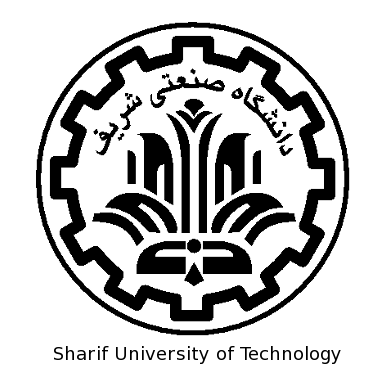
\includegraphics[width=1.1\textwidth]{shariflogo}};
  \end{tikzpicture}%
} 
%%%%%%%%%%%%%%%%%%%%%%%%%%%%%%%%%%%%%%%%%%%%%%%%%%%%%%%%%%%%%%%%%%%%%%%%%%%%%
%% Here starts the poster
%%---------------------------------------------------------------------------
%% Format it to your taste with the options
%%%%%%%%%%%%%%%%%%%%%%%%%%%%%%%%%%%%%%%%%%%%%%%%%%%%%%%%%%%%%%%%%%%%%%%%%%%%%
      \definecolor{silver}{cmyk}{0,0,0,0.3}
      \definecolor{yellow}{cmyk}{0,0,0.9,0.0}
      \definecolor{reddishyellow}{cmyk}{0,0.22,1.0,0.0}
      \definecolor{black}{cmyk}{0,0,0.0,1.0}
      \definecolor{darkYellow}{cmyk}{0,0,1.0,0.5}
      \definecolor{darkSilver}{cmyk}{0,0,0,0.1}

      \definecolor{lightyellow}{cmyk}{0,0,0.3,0.0}
      \definecolor{lighteryellow}{cmyk}{0,0,0.1,0.0}
      \definecolor{lighteryellow}{cmyk}{0,0,0.1,0.0}
      \definecolor{lightestyellow}{cmyk}{0,0,0.05,0.0}

      \begin{poster}%
      % Poster Options
      {
      eyecatcher=true,
      % Color style
      bgColorOne=lightyellow,
      bgColorTwo=yellow,
      borderColor=reddishyellow,
      headerColorOne=yellow,
      headerColorTwo=reddishyellow,
%      headerFontColor=silver,
      boxColorOne=red,
      boxColorTwo=lighteryellow,
      % Format of textbox
      textborder=faded,
      % Format of text header
      headerborder=closed,
      headerheight=0.1\textheight,
      headershape=roundedleft,
      headershade=plain,
%      headerfont=\Large, %Sans Serif
      boxshade=shadetb,%plain,
      background=user,%plain,
      linewidth=2pt,
      grid=false,
      }
 % Eye Catcher
 {
      
\includegraphics[height=0.07\textheight]{logo}
 }
 % Title
 {عنوان پوستر عنوان پوستر عنوان پوستر عنوان پوستر عنوان پوستر عنوان پوستر عنوان پوستر 
}
 % Authors
 {\large نام۱ نام خانوادگی۱, نام۳ نام خانوادگی۲, نام۳ نام خانوادگی۳ 
 \\%[1em]
 {\normalsize\texttt{\lr{name1@mail.org, name2@mail.edu, name3@mail.com}}}}
 % University logo
 {
\begin{tabular}{r}
    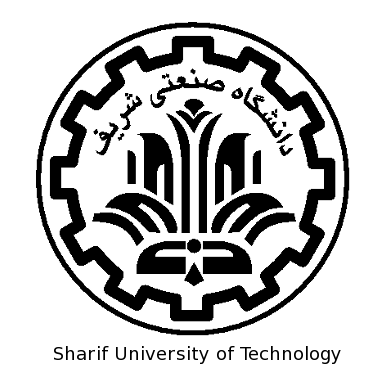
\includegraphics[height=0.07 \textheight]{shariflogo}\\
\end{tabular}
 }

%%%%%%%%%%%%%%%%%%%%%%%%%%%%%%%%%%%%%%%%%%%%%%%%%%%%%%%%%%%%%%%%%%%%%%%%%%%%%%
%%% Now define the boxes that make up the poster
%%%---------------------------------------------------------------------------
%%% Each box has a name and can be placed absolutely or relatively.
%%% The only inconvenience is that you can only specify a relative position 
%%% towards an already declared box. So if you have a box attached to the 
%%% bottom, one to the top and a third one which should be inbetween, you 
%%% have to specify the top and bottom boxes before you specify the middle 
%%% box.
%%%%%%%%%%%%%%%%%%%%%%%%%%%%%%%%%%%%%%%%%%%%%%%%%%%%%%%%%%%%%%%%%%%%%%%%%%%%%%

 %%%%%%%%%%%%%%%%%%%%%%%%%%%%%%%%%%%%%%%%%%%%%%%%%%%%%%%%%%%%%%%%%%%%%%%%%%%%%%
\begin{posterbox}[name=introduction,column=0,row=0]{\textxecolor{red}{مقدمه}}
 %%%%%%%%%%%%%%%%%%%%%%%%%%%%%%%%%%%%%%%%%%%%%%%%%%%%%%%%%%%%%%%%%%%%%%%%%%%%%%
برای تست بسته سعی می‌کنم که یک خط فارسی بنگارم\LTRfootnote{test} تا نتیجه آن را در این پوستر مشاهد کنم\footnote{تست پانویسی}.
\end{posterbox}
 %%%%%%%%%%%%%%%%%%%%%%%%%%%%%%%%%%%%%%%%%%%%%%%%%%%%%%%%%%%%%%%%%%%%%%%%%%%%%%
\begin{posterbox}[name=phase2,column=1,span=1]{فاز دو: پردازش}
 %%%%%%%%%%%%%%%%%%%%%%%%%%%%%%%%%%%%%%%%%%%%%%%%%%%%%%%%%%%%%%%%%%%%%%%%%%%%%%

\begin{wrapfigure}{r}{.6\textwidth}
%\centering
%  \vspace{-10pt}
%{
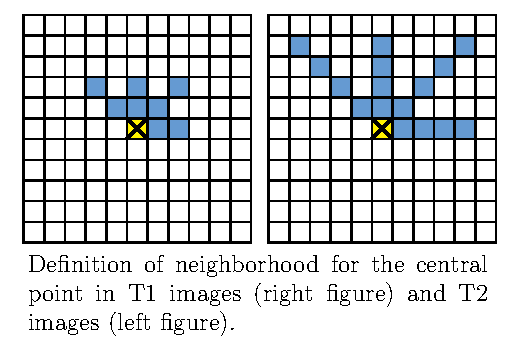
\includegraphics[scale=.5]{fig3}
%}
%  \vspace{-20pt}
\end{wrapfigure}

\ptext[2]

محاسبات لازم:
\begin{align*}
f_1 &= \frac{HXY-HXY1}{max\{HX,HY\}}\\
f_2 &= \sqrt{1-\exp\{-2(HXY2-HXY)\}} 
\end{align*}

{\scriptsize 
\centerline{\begin{minipage}{.95\textwidth}
C(i, j) is an element of GLC matrix and N is number of gray-levels.
\end{minipage}}
\vspace{-.5mm}
$$\begin{array}{l}

\displaystyle C_x(i) =\sum_{j=1}^N C(i,j), \quad C_y(i)=\sum_{i=1}^N C(i,j)\\
\displaystyle  HXY = -\sum_{i=1}^N\sum_{j=1}^N C(i,j) \log\{C(i,j)\}\\
\displaystyle  HXY1 = -\sum_{i=1}^N\sum_{j=1}^N C(i,j) \log\{C_x(i)\times C_y(j)\}\\
\displaystyle  HXY2 = -\sum_{i=1}^N\sum_{j=1}^N C_x(i)\times C_y(j) \log\{C_x(i)\times C_y(j)\}\\
\end{array}$$
}
\end{posterbox}

 %%%%%%%%%%%%%%%%%%%%%%%%%%%%%%%%%%%%%%%%%%%%%%%%%%%%%%%%%%%%%%%%%%%%%%%%%%%%%%
\begin{posterbox}[name=phase3,column=2,span=1,row=0]{استخراج ویژگی‌های: دوتایی}
 %%%%%%%%%%%%%%%%%%%%%%%%%%%%%%%%%%%%%%%%%%%%%%%%%%%%%%%%%%%%%%%%%%%%%%%%%%%%%%
\ptext[7]
\centerline{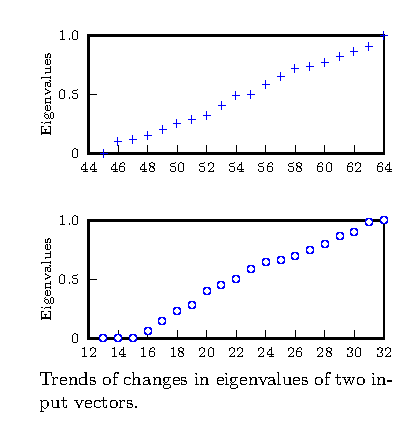
\includegraphics[scale=1.1,height=7cm]{fig4}}
\end{posterbox}

 %%%%%%%%%%%%%%%%%%%%%%%%%%%%%%%%%%%%%%%%%%%%%%%%%%%%%%%%%%%%%%%%%%%%%%%%%%%%%%
\begin{posterbox}[name=phase4,column=2,span=1,below=phase3]{جداسازی}
 %%%%%%%%%%%%%%%%%%%%%%%%%%%%%%%%%%%%%%%%%%%%%%%%%%%%%%%%%%%%%%%%%%%%%%%%%%%%%%
\ptext[6]
\end{posterbox}
 %%%%%%%%%%%%%%%%%%%%%%%%%%%%%%%%%%%%%%%%%%%%%%%%%%%%%%%%%%%%%%%%%%%%%%%%%%%%%%
\begin{posterbox}[name=results,column=1,span=2,below=phase2]{نتایج}
 %%%%%%%%%%%%%%%%%%%%%%%%%%%%%%%%%%%%%%%%%%%%%%%%%%%%%%%%%%%%%%%%%%%%%%%%%%%%%%
\begin{multicols}{2}
    \centerline{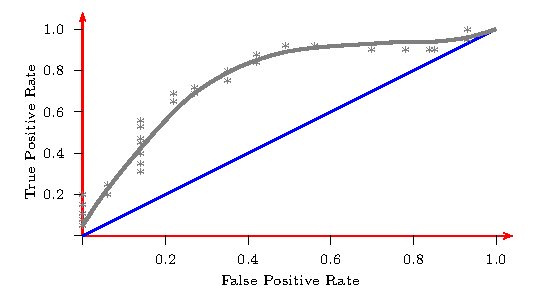
\includegraphics[scale=.7]{fig6}}
    \ptext[2-3]
    
    \centerline{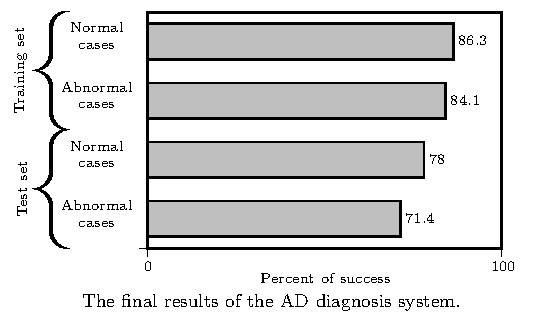
\includegraphics[scale=.7]{fig5}}
\end{multicols}
\end{posterbox}
%%%%%%%%%%%%%%%%%%%%%%%%%%%%%%%%%%%%%%%%%%%%%%%%%%%%%%%%%%%%%%%%%%%%%%%%%%%%%%
\begin{posterbox}[name=imagedataset,column=0,span=1,below=introduction]{پایگاه داده تصاویر}
 %%%%%%%%%%%%%%%%%%%%%%%%%%%%%%%%%%%%%%%%%%%%%%%%%%%%%%%%%%%%%%%%%%%%%%%%%%%%%%
\begin{itemize}
	\item ۱۱۰ تصویر سالم
	\item ۶۶ تصویر ناسالم
	\item ۶۰ درصد تصاویر برای آموزش به کار برده شده‌اند و مابقی برای تست درستی الگوریتم.
	\item وبسایت \url{http://www.med.harvard.edu/AANLIB/home.html}
\end{itemize}
\end{posterbox}
 %%%%%%%%%%%%%%%%%%%%%%%%%%%%%%%%%%%%%%%%%%%%%%%%%%%%%%%%%%%%%%%%%%%%%%%%%%%%%%
\begin{posterbox}[name=phase1,column=0,span=1,below=imagedataset]{فاز یک{:} پیش‌پردازش}
 %%%%%%%%%%%%%%%%%%%%%%%%%%%%%%%%%%%%%%%%%%%%%%%%%%%%%%%%%%%%%%%%%%%%%%%%%%%%%%
\ptext[12]
\begin{enumerate}
	\item پشت زمینه
	\item زنگ روشن
	\item بخش‌های نامرتبط
\end{enumerate}
\ptext[14]

برای هر $\lambda \geq 0$ ورودی نیمه‌مثبت $x\in R^m$ صحیح به‌دست می‌آید البته اگر برای $\lambda X$، $\lambda Y$ ($\lambda >0$) آنگاه ($\lambda y$ و $\lambda x$)

\ptext[16-17]
\end{posterbox}
%%%%%%%%%%%%%%%%%%%%%%%%%%%%%%%%%%%%%%%%%%%%%%%%%%%%%%%%%%%%%%%%%%%%%%%%%%%%%%
\begin{posterbox}[name=adhoc,column=0,span=1,below=phase1]{همینطوری}
 %%%%%%%%%%%%%%%%%%%%%%%%%%%%%%%%%%%%%%%%%%%%%%%%%%%%%%%%%%%%%%%%%%%%%%%%%%%%%%
\textxecolor{red}
{برای پر کردن فضا استفاده شده است. برای پر کردن فضا استفاده شده است. برای پر کردن فضا استفاده شده است. 
برای پر کردن فضا استفاده شده است. برای پر کردن فضا استفاده شده است. برای پر کردن فضا استفاده شده است. 
سلام}
\end{posterbox}
%%%%%%%%%%%%%%%%%%%%%%%%%%%%%%%%%%%%%%%%%%%%%%%%%%%%%%%%%%%%%%%%%%%%%%%%%%%%%%
\begin{posterbox}[name=references,column=1,span=2,below=results]{منابع}
 %%%%%%%%%%%%%%%%%%%%%%%%%%%%%%%%%%%%%%%%%%%%%%%%%%%%%%%%%%%%%%%%%%%%%%%%%%%%%%
     \smaller
%     \bibliographystyle{ieee}
     \renewcommand{\section}[2]{\vskip 0.05em}
       \begin{thebibliography}{1}\itemsep=-0.01em
       \setlength{\baselineskip}{0.4em}
       \bibitem{}
       محمود سیستانی, سیدجواد علوی, رضا حسینی
	, ''بررسی پوستر در فضای فارسی``
	, کنفرانس سالانه کامپیوتر, صفحات 868--871, بهار ۱۳۹۲.
       \end{thebibliography}
\end{posterbox}
 %%%%%%%%%%%%%%%%%%%%%%%%%%%%%%%%%%%%%%%%%%%%%%%%%%%%%%%%%%%%%%%%%%%%%%%%%%%%%%
\begin{posterbox}[name=ack,column=0,span=2,below=references]{قدردانی}
 %%%%%%%%%%%%%%%%%%%%%%%%%%%%%%%%%%%%%%%%%%%%%%%%%%%%%%%%%%%%%%%%%%%%%%%%%%%%%%
با تشکر از دکتر \lr{Brian Amberg}؛ این کار فارسی‌سازی پوستری است که توسط ایشان طراحی شده است\footnote{\url{http://www.brian-amberg.de/uni/poster/}}.
\end{posterbox}
 %%%%%%%%%%%%%%%%%%%%%%%%%%%%%%%%%%%%%%%%%%%%%%%%%%%%%%%%%%%%%%%%%%%%%%%%%%%%%%
\begin{posterbox}[name=ack,column=2,span=1,below=references]{خالی}
 %%%%%%%%%%%%%%%%%%%%%%%%%%%%%%%%%%%%%%%%%%%%%%%%%%%%%%%%%%%%%%%%%%%%%%%%%%%%%%
فضای خالی فضای خالی فضای خالی فضای خالی فضای خالی فضای خالی فضای خالی فضای خالی فضای خالی فضای خالی 
فضای خالی فضای خالی فضای خالی فضای خالی فضای خالی فضای خالی فضای خالی فضای خالی فضای خالی فضای خالی 
\end{posterbox}%%
\end{poster}

\end{document}
